\section{Dust detection algorithms}

onboard algorithom and introduce CNN and how cnn performs

\section{Orbital parameters and the data set}

The trajectory (region, speed, inclination) is important. We will examine SolO and PSP separately, since they are a bit different.

\subsection{Solar Orbiter}

orbits and orbital paramters of SolO to describe what is in the data and what we could have done and what we could not have done. eg escaping population is apparent (beta), but we could never detect ISD due to the alignment. also mention SC potential

\subsection{Parker Solar Probe}

again, what could be extracted from the data and what could not. Meniton the potential and that it is a mess











% In this chapter, a brief derivation of the reduced fluid models used in the included publications is presented. The derivations start from the Braginskii fluid equations whose assumptions and validity for SOL plasmas are discussed. Applying drift reduction, Bohm-normalization and a number of approximations, results in the reduced two-fluid model, equivalent to the two-dimensional fluid models used in Paper III and IV. By applying interchange normalization this model will be further modified to the idealized interchange model, used in Paper I. 

% \section{Braginskii fluid equations}
% The Braginskii fluid model is derived by taking successive velocity moments of the kinetic Boltzmann equation and applying a collisional closure. Each moment depends on the next higher order and therefore require additional assumptions to obtain a closure for the model. The Braginskii equations describe the evolution of the three lowest order fluid moments. The assumptions and the formulation of this closure are presented in \cite{braginskii}. The standard Braginskii fluid equations describing the evolution of the particle density $n_\alpha$, fluid velocity $\textbf{u}_\alpha$ and temperature $T_\alpha$ for particle species $\alpha$ are given by 
% \begin{equation}\label{brag_1}
% 	\frac{\partial n_\alpha}{\partial t} + \nabla \cdot (n_\alpha \textbf{u}_\alpha) = 0,
% \end{equation}
% \begin{equation}\label{brag_2}
% 	m_\alpha n_\alpha \left(\frac{\partial}{\partial t} + \textbf{u}_\alpha \cdot \nabla\right)\textbf{u}_\alpha = - \nabla p_\alpha - \nabla \cdot \Pi_\alpha +Z_\alpha e n_\alpha\left(\textbf{E} + \textbf{u}_\alpha \times \textbf{B}\right) + \textbf{R}_\alpha ,
% \end{equation}
% \begin{equation}\label{brag_3}
% 	\frac{3}{2}n_\alpha \left(\frac{\partial}{\partial t} + \textbf{u}_\alpha \cdot \nabla\right)T_\alpha + p_\alpha \nabla \textbf{u}_\alpha = - \nabla \cdot \textbf{q}_\alpha - \Pi_\alpha : \nabla \textbf{u}_\alpha + Q_\alpha.
% \end{equation}

% Here, $\alpha$ determines the particle species, i.e., electrons and ions, $m$ the particle mass, $p$ the pressure, $Z_\alpha e$ the particle charge, $\textbf{R}$ the friction force, $\Pi$ the viscous stress tensor, $\textbf{q}$ the heat flux, : the tensor inner product and $Q$ the frictional interspecies heating and energy exchange.%, and $S$, $\textbf{S}$ and $W$ represent local density, momentum and energy sources, respectively.
% %In the following, we will focus on the first two moments as all models used in the included papers are isothermal. 

% The Braginskii equations are only applicable if certain assumptions for the modeled system are valid. Applying fluid equations requires that the distribution of particle velocities is close to Maxwellian, i.e., the time scale of relaxation back to a Maxwellian must be shorter than the characteristic time scales of the modeled system. If this condition is fulfilled, the system is referred to as collisional. %This can be expressed as $\omega_c \ll \nu_{ei}$ and $\omega_c \ll \nu_{ii}$ where $\omega_c$ stands for the characteristic frequency of the modeled system and $\nu_{\alpha\beta}$ for the average collision frequency between particle species $\alpha$ and $\beta$. In addition, $l_\parallel \gg \lambda_e$ and $l_\perp \gg \lambda_i$ where $l_\parallel$ and $l_\perp$ represent the smallest length scales of the system parallel and perpendicular to the magnetic field and $\lambda_\alpha$ is the mean free path for a particle species $\alpha$, given by $\lambda_\alpha = v_{\mathrm{th},\alpha}/\nu_{\alpha\beta}$ with the thermal velocity defined as $v_{\mathrm{th},\alpha}= \sqrt{T_\alpha/m_\alpha}$. \textcolor{red}{Ask Fulvio about  i and e}
% In addition to being collisional, a plasma must be strongly magnetized to be adequately described by the Braginskii equations. This implies that the particles complete many gyrations between collisions, setting an upper limit for the collisionality of the plasma. %This condition can be formulated as $\nu_{ie} \ll \Omega_e$ and $\nu_{ii} \ll \Omega_i$ where the gyration frequency is defined as $\Omega_\alpha = eB/m_\alpha$, and $l_\parallel \gg \rho_e$ and $l_\parallel \gg \rho_i$ with the gyration radius given by $\rho_\alpha = v_{\mathrm{th},\alpha}/\Omega_\alpha$. These conditions define the range of time and length scales in which the Braginskii model is valid.

% In summary, the phenomenon we want to model needs to satisfy the following conditions in order to be well described by the Braginskii equations:
% \begin{equation}
% 	L_\perp \gg \rho_\alpha,
% \end{equation}
% \begin{equation}
% 	L_\parallel \gg \lambda,
% \end{equation}
% \begin{equation}
% 	\tau \gg \tau_c \gg \Omega_\alpha^{-1}. 
% \end{equation}
% In these expressions $L_\perp$ stands for the characteristic size of the modeled phenomena perpendicular to the magnetic field, $\rho_\alpha$ is the gyration radius for species $\alpha$, $L_\parallel$ the parallel size of the system, $\lambda$ the collisional mean free path, $\tau$ the characteristic time of the problem, $\tau_c$ the collision time and $\Omega_\alpha$ the gyration frequency of the referred particle species \cite{militellobook}. 

% For the further derivation using drift reduction it will be useful to quantify the magnetization. We thereby define the magnetization parameter $\delta$ as 
% \begin{equation}
% 	\delta = \frac{\rho_\alpha}{L_\perp}.
% \end{equation}
% The magnetization can be equivalently expressed in the temporal domain by 
% \begin{equation}
% 	\delta = \frac{\nu_{ie}}{\Omega_i}
% \end{equation}
% where $\nu_{ie}$ stands for the collisional frequency between ions and electrons.

% For both electrons and ions the magnetization parameter is $\delta \ll 1$ for a fully magnetized plasma. 


% \section{Drift reduction}
% The Braginskii model given by \Eqsref{brag_1} - \eqref{brag_3} is very general, making modeling of SOL plasmas with the presented equations relatively inefficient. A more suitable description of plasma phenomena in the SOL can be derived by simplifying the presented model with an approach called drift ordering. Since turbulence and filaments in the SOL, evolve with velocities much lower than the plasma sound speed $c_s = \sqrt{(T_e+T_i)/m_i}$ we apply the ordering
% \begin{equation}
% 	\textbf{u}_\perp \sim \frac{\rho_\alpha}{L_\perp} c_s \sim \delta c_s.
% \end{equation}
% This ordering assumes that the transverse electric fields are small, resulting in the perpendicular electric field being substantially electrostatic. This is a direct consequence of the $\textbf{E}\times\textbf{B}$ velocity being a factor $\delta$ smaller than sound speed and Faraday's law \cite{militellobook}. We can now determine the perpendicular part of the momentum equation, given by \Eqref{brag_2}, by taking the cross product with $\textbf{B}$ resulting in
% \begin{equation}
% 	\textbf{u}_{\alpha,\perp} = \frac{\textbf{E}\times\textbf{B}}{B^2} - \frac{\nabla p_\alpha \times \textbf{B}}{e_\alpha n_\alpha B^2} - \frac{m_\alpha d \textbf{u}_\alpha/d t \times \textbf{B}}{e_\alpha B^2} - \frac{\nabla \cdot \Pi_\alpha\times\textbf{B}}{e_\alpha n_\alpha B^2} + \frac{\textbf{R}_\alpha \times \textbf{B}}{e_\alpha n_\alpha B^2},
% \end{equation}
% where we used $d/dt = \partial/\partial t + (\textbf{u}_\alpha\cdot \nabla)$ and assumed single charge particle species, i.e., $Z_\alpha e = e_\alpha$. The terms in this expression display the fluid drifts occurring in the system, namely from left to right: the $\textbf{E}\times\textbf{B}$ drift; the diamagnetic drift; the polarization drift; the viscous drift and the collisional drift. From this expression we can determine the dominant drifts and thereby simplify the model.

% As mentioned previously, the electric drift velocity is of $\mathcal{O}(\delta)$ compared to the plasma sound speed:
% \begin{equation}
% 	\textbf{u}_E = \frac{\textbf{E}\times\textbf{B}}{B^2} \sim \delta c_s.
% \end{equation}
% Similarly, the diamagnetic drift is also of $\mathcal{O}(\delta)$ since
% \begin{equation}
% 	\textbf{u}_{\mathrm{dia}} = -\frac{\nabla p_\alpha \times \textbf{B}}{e_\alpha n_\alpha B^2} \sim \frac{n_\alpha T_\alpha B}{L_\perp e_\alpha n_\alpha B^2} \sim \frac{T_\alpha}{L_\perp \Omega_\alpha m_\alpha} \sim \delta c_s.
% \end{equation}
% The polarization drifts for both ions and electrons are smaller in comparison, as can be shown by
% \begin{equation}
% 	\textbf{u}_{\mathrm{pol},i} = \frac{m_i d \textbf{u}_i/d t \times \textbf{B}}{e_i B^2}  \sim \delta^3 c_s,
% \end{equation}
% and
% \begin{equation}
% 	\textbf{u}_{\mathrm{pol},e} \sim \frac{m_e}{m_i} \delta^3 c_s.
% \end{equation}
% For the viscous drift we use Bragniskii's approximation for the perpendicular component of the viscous stress tensor $\Pi_\alpha \sim (p_\alpha/\Omega_\alpha) \nabla v_{\alpha}$ which shows that this term is of $\mathcal{O}(\delta^3)$ since
% \begin{equation}
% 	\textbf{u}_{\mathrm{vis},i} = \frac{\nabla \cdot \Pi_\alpha\times\textbf{B}}{e_\alpha n_\alpha B^2} \sim \frac{nT \delta c_s}{e_i n_i B L_\perp^2 \Omega} \sim \delta^3 c_s,
% \end{equation}
% and
% \begin{equation}
% 	\textbf{u}_{\mathrm{vis},e} \sim \frac{m_e}{m_i}\delta^3  c_s,
% \end{equation}
% respectively. Lastly, we need to find an approximation for the collisional drift. For this we use $\textbf{R}_\perp = e n\,\textbf{J}_\perp/\sigma_\perp$ for the perpendicular momentum transfer from electron-ion friction and $\sigma_\perp = ne^2\nu_{ei}/m_e$. From the ordering follows $\textbf{J}_\perp \sim en\delta c_s$ which leads to the approximation of the frictional drift 
% \begin{equation}\label{diffusion}
% 	\textbf{u}_{\mathrm{fri}} =\frac{\textbf{R}_\alpha \times \textbf{B}}{e_\alpha n_\alpha B^2} \sim \frac{ne\delta c_s}{B \sigma_\perp} \sim \frac{m_e}{m_i}\frac{\nu_{ei}}{\Omega}\delta c_s.
% \end{equation}
% For SOL conditions we can typically assume that $\nu_{ei}/\Omega\sim \delta$ so that the collisional drift is of  $\mathcal{O}(\delta^2)$. 

% This ordering reveals that the dominant perpendicular drifts are the electric and the diamagnetic drifts as all other drifts are at least one order of magnitude smaller. By substituting the remaining drifts into the Braginskii equation we can rewrite the electron density equation in a simpler form,
% \begin{equation}\label{n_e}
% 	\frac{\partial n_e}{\partial t} + \nabla \cdot\left[n_e\left(\textbf{u}_E + \textbf{u}_{\mathrm{dia},e}+ \textbf{u}_{e \parallel}\right)\right] = 0.
% \end{equation}
% Since the plasma is quasi-neutral, i.e.\ $n_e\simeq n_i\simeq n$, this equation is used to describe the evolution of the total plasma density $n$. \Eqref{n_e} is usually manipulated to
% \begin{equation}\label{dens}
% 	\frac{\partial n}{\partial t} + \textbf{u}_E \cdot \nabla n = -\nabla\cdot\left(n\textbf{u}_{\parallel,e}\right) + \left(\frac{1}{e}\nabla p_e - n \nabla \phi\right)\cdot\nabla\times \left(\frac{\textbf{b}}{B}\right).
% \end{equation}
% %As we can see, the diamagnetic drift does not give rise to plasma advection as this term is not a drift of guiding centers but a consequence of counting particle motion through an area in the fluid picture, leading to so called diamagnetic cancellation inside the divergence terms. In non-uniform magnetic fields, this cancellation results in a non-divergence free term $\nabla \times (\textbf{b}/B)$, referred to as the curvature operator, which will be discussed later. 

% Instead of explicitly deriving separate continuity equations for electrons and ions, we can utilize quasi-neutrality and charge conservation to derive an equation for the fluid velocity, which will prove to be very handy. For this we use $\nabla \cdot \textbf{J} = 0$ with $\textbf{J}= e n (\textbf{u}_i - \textbf{u}_e)$. Inserting all drifts that give rise to a net current results in 
% \begin{equation}\label{diff_J}
% 	\nabla \cdot \left(\textbf{J}_{\mathrm{dia}} + \textbf{J}_{\mathrm{pol}} +\textbf{J}_{\mathrm{vis}}+ \textbf{J}_{\parallel}\right) = 0.
% \end{equation}
% In the following we only include the leading order drifts in the ion polarization velocity and neglect the electron polarization drift entirely due to the small electron mass. The sum of the ion polarization and viscous drifts using the lowest order solution
% of the perpendicular momentum equation and the parallel velocity $\textbf{u}_0 = \textbf{u}_{0\perp} + \textbf{u}_{i\parallel}$ is then given by
% \begin{equation}
% 	\textbf{u}_{\mathrm{pol},i} + \textbf{u}_{\mathrm{vis},i} = \textbf{b}\times \frac{1}{enB}\left[m_i n \left(\frac{\partial}{\partial t} + \textbf{u}_{i0} \cdot \nabla\right)\textbf{u}_{i0} + \nabla \cdot \Pi_{i0}\right],
% \end{equation}
% where $\Pi_{i0}$ is the viscous stress tensor calculated with $\textbf{u}_{i0}$ and
% \begin{equation}
% 	\textbf{u}_{0\perp} = \textbf{b}\times \frac{1}{B}\left(\nabla \phi + \frac{1}{en} \nabla p_i \right).
% \end{equation}
% Inserting this into \Eqref{diff_J} leads to the drift-reduced charge conservation equation  \cite{militellobook}
% \begin{multline}\label{charge_conservation}
% 	-\nabla \cdot \left\{\textbf{b}\times\frac{1}{B} \left[m_i n\left(\frac{\partial}{\partial t} + \textbf{u}_{i0}\cdot \nabla\right)\textbf{u}_{i0} + \nabla\cdot \Pi_{i0}\right]\right\} =\\ \nabla\cdot\textbf{J}_\parallel + \nabla \left(p_i + p_e\right) \cdot \nabla\times \left(\frac{\textbf{b}}{B}\right),
% \end{multline}
% which will be further simplified in the following.
% \section{Further approximations and simplifications}
% A number of additional approximations are applied to simplify the model and make it efficiently numerically solvable. 

% First of all, we apply the {electrostatic} approximation, and thereby neglect all time derivatives of $\textbf{B}$ and calculate the electric field $\textbf{E}$ directly from the electric potential. Under this approximation, \Eqref{charge_conservation} can be expressed in the more readable form
% \begin{multline}\label{electrostatic}
% 	m_{i}\nabla\cdot\left[\frac{n}{B} \frac{d_0}{dt}\left(\frac{\nabla_\perp\phi}{B} + \frac{\nabla_\perp p_i}{enB}\right) \right] - \nabla\cdot \left(\textbf{b}\times \nabla\cdot \Pi_0\right) = 
% 	\\ \nabla\cdot\textbf{J}_\parallel + \nabla\left(p_i + p_e\right)\cdot \nabla\times \left(\frac{\textbf{b}}{B}\right),
% \end{multline}
% where we used $d_0/dt = \partial/\partial t + (\textbf{u}_{i0}\cdot \nabla)$. In addition, we neglected spatial non-uniformity of $\textbf{B}$, which will be discussed in further detail later. Studies of electromagnetic effects on plasma blob-filament transport showed that these effects in high temperature or high beta plasmas suppress the resistive drift wave turbulence in filaments \cite{lee2015electromagnetic,hoare2019dynamics} but will not be considered in the following. 

% We can further simplify \Eqref{electrostatic} by applying scale separation for the plasma density, so that $\nabla n \sim \nabla n_0 + \nabla \widetilde{n} \sim 1/L_n + k \widetilde{n}$, where the particle density has been separated into a background $n_0$ and a fluctuation $\widetilde{n}$. $L_n$ stands for the characteristic scale length for the background density and $k$ for the wave number for the particle density fluctuations. Dividing by $n_0$ leads to $\nabla \ln{n} \sim 1/L_n + k \widetilde{n}/n_0$. We now assume that $1/kL_n \ll 1$ and $\widetilde{n}/n_0 \ll 1$. The latter assumption is the so called {thin layer} or {Boussinesq} approximation where we assume that the density perturbations are small compared to the equilibrium. This assumption is hardly justified since relative fluctuations in the SOL can be of order unity as discussed in the previous chapter. This approximation is, however, commonly used since it makes the numerical integration of \Eqref{electrostatic} significantly more efficient. By introducing a generalized vorticity,
% \begin{equation}
% 	\varpi = \nabla\cdot\left(\nabla_\perp \phi + \frac{\nabla_\perp p_i}{en}\right),
% \end{equation}
% we can now simplify the first term in \Eqref{electrostatic} to
% \begin{equation}
% 	m_{i}\nabla\cdot\left[\frac{n}{B} \frac{d_0}{dt}\left(\frac{\nabla_\perp\phi}{B} + \frac{\nabla_\perp p_i}{enB}\right) \right] \approx \frac{m_i n}{B^2}\frac{d_0\varpi}{dt}.
% \end{equation}
% From this expression, $\varpi$ can be relatively easily inverted, especially when assuming that ions are cold, leading us to the next approximation. 

% For the remaining derivation we will assume {small ion temperature}, $T_i \ll T_e$, simplifying the equations significantly. This is a restrictive assumption, as experimental measurements indicate that the ion temperature is higher than the electron temperature in the SOL \cite{kovcan2007ion,kocan2012ion}. Numerical simulations incorporating finite ion temperature have shown that the coherency of filaments is increased \cite{Ahmed_ions}. However, since the simplified model still captures the fundamental dynamics in the SOL, this approximation is commonly used to reduce the model complexity.

% As for the electrons, all models in the included publications and manuscripts assume {isothermal electrons}. This assumption simplifies the model drastically, as it makes \Eqref{brag_3} obsolete. Numerical simulations of isolated filaments with dynamic electron temperature have shown that thermal effects lead to a strong increase in the filament propagation in the poloidal direction and reduce the net radial propagation. These effects arise from the electron temperature dependence of the sheath currents, which will be discussed later in this chapter \cite{walkden2016dynamics}. 

% Next, we will define the geometry of the magnetic field. For the whole simulation domain, we assume {straight magnetic field} lines with {constant} field strength. We need to make one exception to this assumption, as no curvature term would remain in a completely homogeneous field. As there would be no drive for filament motion without this term, it is required to capture some effects of curvature in the model. With the use of vector algebra presented in \cite{militellobook} we can write the curvature term from \Eqsref{dens} and \eqref{electrostatic} as
% \begin{equation}
% 	\nabla\times\left(\frac{\textbf{b}}{B}\right) = 2\frac{\textbf{b}\times{\boldsymbol\kappa}}{B} + \frac{\mu_0\left(\textbf{J}_\parallel - \textbf{J}_\perp\right)}{B^2},
% \end{equation}
% where we introduced the curvature vector $\boldsymbol\kappa = (\textbf{b}\cdot\nabla)\textbf{b}$. Note that one unit of the term $\textbf{b}\times\boldsymbol\kappa/B$ originates from the magnetic gradient and one from the curvature. The second term on the right hand side can be neglected due to charge conservation \cite{militellobook}. The magnetic field in a tokamak can be approximated to lowest order to be purely toroidal and falling radially with $1/R$. In a cylindrical coordinate system $(R,\Phi,Z)$ the toroidal magnetic field is therefore
% \begin{equation}
% 	\textbf{B} = \frac{B_0R_0}{R}\boldsymbol{\widehat{\Phi}}.
% \end{equation}
% In a slab geometry with Z being replaced with the binormal direction $y$ which is perpendicular to $\widehat{\textbf{R}}$ and $\boldsymbol{\widehat{\Phi}}$ this motivates the definition of the curvature operator
% \begin{equation}\label{curvature}
% 	\mathcal{K}(u) = \nabla\times \left(\frac{\textbf{b}}{B}\right)\cdot\nabla u\approx -\frac{2}{B_0R_0}\frac{\partial u}{\partial y}.
% \end{equation}
% %In this expression $R_0$ is defined as the sum of the major and minor radius and $B_0$ the magnetic field strength at that radial position.

% Despite arguing that the frictional drift is negligible in \Eqref{diffusion} one typically retains an approximation of this term due to numerical reasons. We therefore add this term to \Eqref{dens} as 
% \begin{equation}\label{diffusion}
% 	\nabla\cdot \left(n_e \textbf{u}_{\textrm{fri}}\right) \approx -\nabla\cdot \left(D_n\nabla_\perp n_e\right)\approx-D_n\nabla^2_\perp n_e,
% \end{equation}
% where we introduced the density diffusion coefficient $D_n$ which we assumed to be spatially constant. Similarly, one can derive the diffusion term for \Eqref{electrostatic} from its ion viscosity term, since we can use the approximation
% \begin{equation}
% 	\nabla\cdot \Pi_i = -m_in\mu_\omega\nabla_\perp^2\textbf{u}_E,
% \end{equation}
% where $\mu_\omega$ stands for the effective cross-field kinematic viscosity of the ions. Inserting the electric drift and taking the divergence results in the diffusion term for $\nabla_\perp^2\phi$ as
% \begin{equation}
% 	\nabla\cdot\left(\frac{m_i \mu_\omega}{eB^2} \nabla_\perp\nabla_\perp^2\phi\right).
% \end{equation}
% The diffusion coefficients can be approximated from classical or neo-classical diffusion such as presented in \cite{fundamenski2007dissipative}, or are chosen for numerical accuracy and stability. 

% Arguably the starkest simplification of the presented models in this thesis is the restriction to only two dimensions, the plane perpendicular to \textbf{B}. The parallel closure of the model equations is different for closed and open field lines, i.e., whether the simulation domain is located in the SOL or in the edge region. Since the parallel direction plays an important role in the SOL for particle and current dissipation as plasma flows along the magnetic field lines towards the divertor plates, a suitable approximation for the parallel losses is required. This closure is achieved by integrating over the parallel direction where the so-called sheath boundary conditions come into play. In the initial transient period where the plasma vessel is filled and the cold wall surface electrically neutral, electrons will strike the surface at a higher rate than the ions due to their higher speed. This charges the vessel walls negatively which impedes further electron flow towards the surface and results in a thin sheath at material surfaces. Here, the ions shield the electric potential of the surface and the sheath extends a few Debye lengths, $\lambda_D = \sqrt{\epsilon_0T_e/n_ee^2}$, outwards from the surface into the plasma. In this region quasi neutrality is violated since the ion density is higher than the electron density, $n_i > n_e$. The electric current density drawn by the vessel walls is governed by the influx of electrons and ions at the sheath surface. It depends on the potential $\phi$ at the sheath entrance and can be written as
% \begin{equation}\label{parallel_flux}
% 	\textbf{J}_\parallel|_{\mathrm{sheath}} = en_{se}c_s \left[1 - \text{e}^{\Lambda-e{\phi}/{T_e}}\right],
% \end{equation}
% with the plasma density at the sheath edge $n_{se}$, the acoustic speed $c_s$ and the floating potential $\Lambda=\mathrm{ln}\sqrt{m_i/2\pi m_e}$. The first term in the parenthesis is due to the ion flux and the second due to the electron flux \cite{stangeby2000plasma}. %Note that while the ion flux at the sheath edge is given by $n_{se}c_s$, the electron flux is dependent on the potential drop in the sheath \cite{stangeby2000plasma}. 
% We can now take the average of the parallel dimension in a slab geometry with $\textbf{B} = B\, \widehat{\textbf{z}}$,
% \begin{equation}\label{v_parallel}
% \frac{1}{L_\parallel} \int_{-L_\parallel/2}^{L_\parallel/2} \nabla_\parallel \cdot \textbf{J}_\parallel dz,
% \end{equation}
% and use \Eqref{parallel_flux} as the boundary conditions. The first term on the right hand side of \Eqref{dens} can be handled analogously for the parallel electron velocity. 

% Paper III includes a core region in the simulation domain, requiring a different closure for the parallel dynamics. In this model we include resistivity in the parallel component of the electron momentum equation neglecting inertia, i.e.,
% \begin{equation}\label{par}
% 	en\frac{\partial\phi}{\partial z} - T_e\frac{\partial n}{\partial z} + \chi enJ_\parallel=0,
% \end{equation}
% where the resistivity is given by $\chi = m\nu_{ei}/n_e e^2$. %We neglect the parallel ion momentum since the ions remain to lowest order stationary due to their high inertia. 
% Rearranging \Eqref{par} for $J_\parallel$ and taking the parallel derivative results in \cite{bellan2008fundamentals,meyer_thesis}
% \begin{equation}\label{resistivity}
% 	\nabla_\parallel \cdot \textbf{J}_\parallel = \frac{T_e}{e\chi}\frac{\partial^2}{\partial z^2}\left(\mathrm{ln}\,n_e - \frac{e\phi}{T_e}\right).
% \end{equation}
% From this we can take the average of the parallel dimension by integrating over $z$, resulting in the desired 2D model equations. A systematic analysis of the dimensionality of scrape-off layer turbulence is presented in \cite{nicholas_dim,Nicholas2021comparing}.

% \section{Reduced two-fluid model}

% Since the Braginskii fluid model is only valid in a specific range of time and length scales it seems natural to normalize all physical variables to values that are characteristic for the modeled system. We will first discuss the so-called Bohm normalization where we normalize the spatial and temporal units by $\rho_s$ and $\Omega_i$, respectively, i.e.,
% \begin{equation}
% 	\nabla \rightarrow \nabla' = \rho_s\nabla, \,\,\, \frac{\partial}{\partial t} \rightarrow \frac{\partial}{\partial t'} = \frac{1}{\Omega_i}\frac{\partial}{\partial t}.
% \end{equation}
% Here, $\rho_s$ stands for the ion sound Larmor radius defined as $\rho_s = \sqrt{T_e m_i}/eB$.
% We normalize the remaining variables with their characteristic values for SOL conditions $N$ and $T_0$ as
% \begin{equation}
% 	n \rightarrow n' = \frac{n}{N},\,\,\, T_e \rightarrow T' = \frac{T_e}{T_0},\,\,\,\phi \rightarrow \phi' = \frac{e\phi}{T_0}. 
% \end{equation}
% From these expressions we can define the characteristic magnitude for the density source, diffusion coefficients and effective gravity drive as
% \begin{equation}
% 	S\rightarrow S' = SN\Omega_i,\,\,\,D_n\rightarrow D_n' = D_{\textrm{Bohm}}D_n,\,\,\,\mu_\omega\rightarrow D_\Omega' = D_{\textrm{Bohm}}\mu_\omega,\,\,\,g = \frac{2\rho_s}{R},
% \end{equation} 
% where the collisional diffusion is defines as $D_{\textrm{Bohm}}= \rho_s^2\Omega_i$. Applying this normalization to \Eqref{dens} and dropping the dash sign, inserting the curvature operator from \Eqref{curvature} and adding the diffusion term of \Eqref{diffusion} results in the electron density equation
% \begin{equation}
% 	\frac{\mathrm{d}n}{\mathrm{d}t} + g \left(\frac{\partial n}{\partial y} - n\frac{\partial\phi}{\partial y}\right) = D_n \nabla_\perp^2 n + S_n + \Bigg \langle \nabla_\parallel \left(n{u}_{e\parallel} \right)\Bigg \rangle_\parallel,
% \end{equation}
% where the advective derivative is given by $\mathrm{d}/\mathrm{d}t = \partial/\partial t + \textbf{u}_E\cdot \nabla_\perp$ and $\textbf{u}_E = - \nabla_\perp\phi\times\textbf{B}/B^2$ is the $\textbf{E}\times\textbf{B}$ drift. Here, $\langle\cdot\rangle_\parallel$ refers to the average over the parallel dimension. We also added the density source term $S_n$. Performing the same kind of operations on \Eqref{electrostatic} after applying the Boussinesq approximation results in the vorticity equation
% \begin{equation}
% 	\frac{\mathrm{d}\nabla_\perp^2 \phi}{\mathrm{d}t} + \frac{g}{n}\frac{\partial n}{\partial y} = D_{\Omega}\nabla_\perp^4 \phi + \Bigg \langle \frac{1}{n} \nabla_\parallel J_{\parallel} \Bigg \rangle_\parallel,
% \end{equation}
% where we introduced $D_{\Omega}$  as the collisional dissipation term representing viscosity. Averaging over the parallel direction after inserting \Eqref{v_parallel} and \Eqref{resistivity} can be expressed as
% \begin{subequations}
% 	\begin{gather}
% 		\Bigg \langle \nabla_\parallel \left(n{u}_{e\parallel} \right) \Bigg \rangle_\parallel = - \eta(x) n\,\exp(\Lambda-\phi) + \chi(x)( \widehat{\phi} - \widehat{n} ) ,
% 		\\
% 		\Bigg \langle \frac{1}{n} \nabla_\parallel J_{\parallel} \Bigg \rangle_\parallel =  \eta(x) \left[ 1-\exp(\Lambda-\phi) \right] + \chi(x)( \widehat{\phi} - \widehat{n} ),
% 	\end{gather}
% \end{subequations}
% where the spatially fluctuating electron density $\widehat{n}$ and plasma potential $\widehat{\phi}$ are defined as $\widehat{n}=n-\langle{n}\rangle_y$ and $\widehat{\phi}=\phi-\langle{\phi}\rangle_y$ and $\langle{\cdot}\rangle_y$ refers to the flux surface average. Note, that we neglect $1/n$ in the plasma conductivity term for the vorticity equation, since we assume the plasma density to have small relative fluctuation levels in the edge region and $n \sim 1$. We redefined $\chi = \left(\rho_s/L_\parallel\right)^2(m_i/m_e)(\Omega_s/\nu_{ei})$ as the normalized parallel plasma conductivity where we used $\nabla_\parallel^2 \rightarrow -k^2_\parallel\simeq-L_\parallel^{-2}$ and introduced $\eta=\rho_s/L_\parallel$ as the normalized sheath dissipation coefficient. $\nu_{ei}$ stands for the collision frequency between electrons and ions given by
% \begin{equation}
% 	\nu_{ei} = \frac{\textrm{log}\Lambda_c e^4Z^2n_i}{6\sqrt{2}\pi^{3/2} \epsilon_0^2\sqrt{m_e}T_e^{3/2}},
% \end{equation}
% and the Coulomb logarithm is approximately \cite{militellobook}
% \begin{equation}
% 	\textrm{log}\Lambda_c\approx 18 - \textrm{log}\left[\left(\frac{n_e}{10^{19}}\right)^{1/2}\left(\frac{T_e}{10^3e}\right)^{-3/2}\right].
% \end{equation}
% These parameters depend on the radial position, the sheath dissipation term only occurs in the SOL and the plasma conductivity term is finite in the plasma edge region. A schematic illustration of these two regions in the simulation domain is shown in \Figref{Fig:model}.
% \begin{figure}[t]
% 	\centering
% 	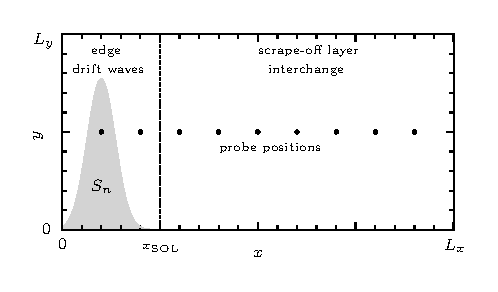
\includegraphics[width=10cm]{figures/model.eps}
% 	\caption{Schematic illustration of the edge and scrape-off layer region in the simulation domain. The position of the plasma
% source term (gray shaded) and the border between edge and SOL (dashed vertical line) are indicated \cite{decristoforo2021numerical}.}
% 	\label{Fig:model}
% \end{figure}

% This model is equivalent to the one used in Paper III. Paper IV utilizes a slightly simpler model placing the whole domain in the SOL by choosing $\eta = \text{constant}$ and $\chi = 0$, and discarding $\Lambda$ in the sheath dissipation term. A list of representative machine parameters relevant for the reduced two-fluid models is presented in Table \ref{tab:machine_parameters}. Since each device performs a range of experiments with slightly different configurations, these parameters might vary. The presented parameters are consistent with those used in the numerical simulations in the included references. The radial position of the SOL is indicated by the sum of the major and minor radius and the parallel connection length is estimated as $L_\parallel = \pi q_{95} R$, with $q_{95}$ as the safety factor  at the 95\% poloidal magnetic flux surface, if not explicitly stated in the references. It should also be noted, that the definition of the connection length varies from source to source as it may refer to the whole poloidal length or only to the lenth between the outboard midplane to the outer divertor plates. 

% \begin{table}[h!]
% 	\begin{center}
% 		\caption{Machine parameters.}
% 		\label{tab:machine_parameters}
% 		\begin{tabular}{c|c c c c c|c} 
% 			 & $n_e[\mathrm{m}^{-3}]$ & $T_e[\mathrm{eV}]$ & $B[\mathrm{T}]$ & $L_\parallel[\mathrm{m}]$ & $R+r[\mathrm{m}]$ & reference\\
% 			\hline
% 			MAST & $8\times 10^{18}$ & 40 & 0.5 & 30 & 1.5 & \cite{easy2016investigation}\\
% 			C-Mod & $1.4\times 10^{19}$ & 23 & 4.5 & 20 & 0.9 & \cite{terry2003observations}\\
% 			TCV & $5\times 10^{18}$ & 25 & 1.45 & 15 & 1.13  & \cite{nespoli2017blob,wensing2019solps}\\
% 			KSTAR & $7\times 10^{17}$ & 35 & 2.0 & 26 & 2.3 & \cite{bak2015investigation} \\
% 			AUG & $8\times 10^{18}$ & 40 & 2.5 & 25 & 2.15 & \cite{militello2011multi} \\
% 			JET & $2\times 10^{19}$ & 45 & 3.45 & 25 & 4.21 & \cite{fundamenski2007dissipative}\\
% 			NSTX & $6\times 10^{18}$ & 13 & 0.25 & 20 & 1.53 & \cite{terry2003observations}
% 		\end{tabular}
% 	\end{center}
% \end{table} 
% The plasma parameters calculated for these device parameters are presented in Table \ref{tab:plasma}.
% \begin{table}[h!]
% 	\begin{center}
% 		\caption{Physical parameters.}
% 		\label{tab:plasma}
% 		\begin{tabular}{c|c c c c} 
% 		 & $\rho_s[\mathrm{m}]$ &$\Omega_i[\mathrm{s}^{-1}]$&$c_s[\mathrm{ms}^{-1}]$\\
% 			\hline
% 			MAST & $1.8\times 10^{-3}$ & $2.4\times 10^{7}$ & $4.4\times 10^{4}$\\
% 			C-Mod& $1.5\times 10^{-4}$ & $2.2\times 10^{8}$ & $3.3\times 10^{4}$\\
% 			TCV & $5.0\times 10^{-4}$ & $6.9\times 10^{7}$ & $3.5\times 10^{4}$\\
% 			KSTAR & $4.3\times 10^{-4}$ & $9.6\times 10^{7}$ & $4.1\times 10^{4}$\\
% 			AUG & $3.7\times 10^{-4}$ & $1.2\times 10^{8}$ & $4.4\times 10^{4}$\\
% 			JET & $2.8\times 10^{-4}$ & $1.7\times 10^{8}$ & $4.6\times 10^{4}$\\
% 			NSTX & $2.1\times 10^{-3}$ & $1.2\times 10^{7}$ & $2.5\times 10^{4}$\\
% 		\end{tabular}
% 	\end{center}
% \end{table}
% Based on these values, we can estimate the input parameters for the reduced two-fluid model shown in Table \ref{tab:input}. Note that the diffusion and viscosity coefficients for the model are not presented as they are chosen arbitrarily high for numerical stability in the included publications.
% \begin{table}[h!]
% 	\begin{center}
% 		\caption{Input parameters.}
% 		\label{tab:input}
% 		\begin{tabular}{c|c c c } 
% 			&  $g$ & $\eta$ & $\chi$ \\
% 			\hline
% 			MAST & $2.4\times 10^{-3}$ &  $6.1\times 10^{-5}$ & $2.7 \times 10^{-4}$\\
% 			C-Mod& $3.4\times 10^{-4}$ &  $7.7\times 10^{-6}$ & $1.0 \times 10^{-5}$\\
% 			TCV & $8.8\times 10^{-4}$ &  $3.3\times 10^{-5}$ & $1.9 \times 10^{-4}$ \\
% 			KSTAR & $3.7\times 10^{-4}$ & $1.6\times 10^{-5}$ & $6.8 \times 10^{-4}$ \\
% 			AUG & $3.4\times 10^{-4}$ & $1.5\times 10^{-5}$ & $7.7 \times 10^{-5}$ \\
% 			JET & $1.3\times 10^{-4}$ & $1.1\times 10^{-5}$ & $3.1 \times 10^{-5}$ \\
% 			NSTX & $2.7\times 10^{-3}$ & $1.0\times 10^{-4}$ & $1.1 \times 10^{-4}$ \\
% 		\end{tabular}
% 	\end{center}
% \end{table}

% \section{Idealized interchange model}
% A minimal model for SOL plasma dynamics in the cross-field plane can be obtained by ignoring parallel dynamics entirely and applying the so called interchange normalization. We start again with \Eqref{dens} and \Eqref{electrostatic}, use the curvature operator given by \Eqref{curvature}, and include the diffusion terms. The perpendicular components then take the form
% \begin{subequations}
% 	\begin{gather}
% 		\left(\frac{\partial}{\partial t} + \frac{1}{B}\widehat{\textbf{z}}\times \nabla\phi\cdot\nabla\right) n - \frac{2n}{B_0 R_0}\frac{\partial \phi}{\partial y} + \frac{2T_e}{eB_0R_0}\frac{\partial n}{\partial y} = D_n\nabla_\perp^2 n,
% 		\\
% 		 \left(\frac{\partial}{\partial t} + \frac{1}{B}\widehat{\textbf{z}}\times \nabla\phi\cdot\nabla\right)\nabla_\perp^2\phi + \frac{2c_s^2}{R_0n}\frac{\partial n}{\partial y} = D_\Omega\nabla_\perp^4 \phi.
% 	\end{gather}
% \end{subequations}
% Under the interchange normalization, length scales are normalized by the characteristic length $l$ of the system, time scales by the ideal interchange rate $\gamma = \sqrt{g/l}$ with $g=2c_s^2/R_0$ and the plasma density and electrostatic potential accordingly, i.e.,
% \begin{equation}
% 	\nabla \rightarrow \nabla' = l\nabla, \,\,\, \frac{\partial}{\partial t} \rightarrow \frac{\partial}{\partial t'} = \frac{1}{\gamma}\frac{\partial}{\partial t}, \,\,\,n \rightarrow n' = \frac{n}{N},\,\,\,\phi \rightarrow \phi' = \frac{\phi}{\gamma B_0l^2}.
% \end{equation}
% Inserting these expressions into the equations for plasma density and vorticity results in 
% \begin{subequations}
% 	\begin{gather}
% 		\left(\frac{\partial}{\partial t'} + \widehat{\textbf{z}}\times \nabla'\phi'\cdot\nabla'\right) n' - 2n'\frac{l}{R_0}\frac{\partial \phi'}{\partial y'} + \frac{\gamma}{\Omega_i}\frac{\partial n'}{\partial y'} = \frac{D_n}{\gamma l^2}{\nabla'}_\perp^2 n',
% 		\\
% 		\left(\frac{\partial}{\partial t'} + \widehat{\textbf{z}}\times \nabla'\phi'\cdot\nabla'\right){\nabla'}_\perp^2\phi' + \frac{1}{n'}\frac{\partial n'}{\partial y'} = \frac{D_\Omega}{\gamma l^2}{\nabla'}_\perp^4 \phi'.
% 	\end{gather}
% \end{subequations}
% We neglect the term resulting from the compression of the electric drift since its prefactor is $l/R_0 \ll 1$. The term resulting from the compression of the diamagnetic drift will also be neglected in the continuity equation as previous work has shown that it has a negligible contribution to the cross-field dynamics and since $\gamma/\Omega_i \ll 1$ \cite{Garcia_thesis}. In addition we introduce the normalized particle diffusion and viscosity coefficients
% \begin{equation}
% 	\kappa = D_n/\gamma l^2 \,\,\,\text{and}\,\,\, \mu = D_\phi/\gamma l^2,
% \end{equation}
% neglect $1/n$ in front of the interchange term as we apply the Boussinesq approximation and drop the dash notation to receive the minimal model for plasma convection 
% \begin{subequations}
% 	\begin{gather}
% 		\left(\frac{\partial}{\partial t} + \widehat{\textbf{z}}\times \nabla\phi\cdot\nabla\right) n = \kappa\nabla_\perp^2 n,
% 		\\
% 		\left(\frac{\partial}{\partial t} + \widehat{\textbf{z}}\times \nabla\phi\cdot\nabla\right)\nabla_\perp^2\phi + \frac{\partial n}{\partial y} = \mu\nabla_\perp^4 \phi.
% 	\end{gather}
% \end{subequations}
% The emphasis of this model lies on reducing the complexity and the number of free parameters as drastically as possible without losing the capability of modeling plasma advection self-consistently. This model has also been used in the past to describe buoyancy-driven convection in a fluid confined between two horizontal plates and heated from below. The model, named the Rayleigh-Bénard convection model after the original experimental work of Henri Bénard \cite{benard1901tourbillons} and the first analytical work on this model of Lord Rayleigh \cite{rayleigh1916lix}, has become a paradigm to investigate nonlinear phenomena due to its rich dynamics \cite{decristoforo2020intermittent, busse1978non,siggia1994high,bodenschatz2000recent,kadanoff2001turbulent,ahlers2009heat}. The normalized particle diffusion and viscosity coefficients in the presented formulation are related to the Rayleigh and Prandtl numbers as $R = 1/\kappa\mu$ and $R=\mu/\kappa$, which are typically used as model parameters for the Rayleigh-Bénard model. We use this model in Paper I.

